\subsection{Attori} \label{Attori}

\begin{figure}[ht]
    \centering
    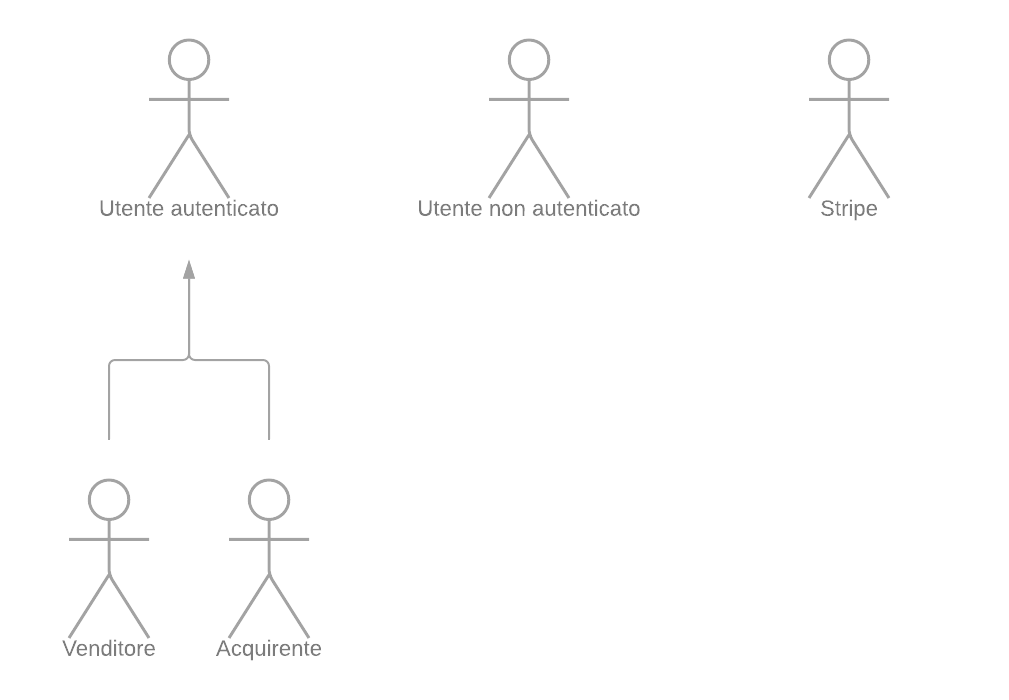
\includegraphics[width=\textwidth]{Immagini/DiagrammiUC/Attori.png}
    \caption{Gerarchia degli utenti} 
    \label{fig:Registrazione}
\end{figure}

\subsubsection{Attori Primari}
\begin{itemize}
    \item \textbf{Utente non autenticato:} utente che può consultare la parte pubblica del sito cercando prodotti e aggiungendoli al carrello, oppure fare il login o registrarsi come acquirente al sito. Non può fare però acquisti sulla piattaforma.
    \item \textbf{Utente autenticato:}
    \begin{itemize}
        \item \textbf{\glo{Acquirente}:} utente che può fare tutto ciò che fa l'utente non autenticato dopo aver effettuato la login o la registrazione. Può effettuare acquisti comprando i prodotti che ha nel carrello, consultare gli ordini che ha fatto, modificare il suo profilo e eseguire il logout.
        \item \textbf{Venditore:} utente che può aggiungere, modificare ed eliminare i prodotti dalla piattaforma, oltre a poter consultare gli ordini fatti dagli acquirenti.
    \end{itemize}
    \item \textbf{Amministratore:} l'amministratore è in grado di fare il \glo{Deploy} dell'applicazione sul \glo{cloud}, configurare le integrazioni di componenti di terze parti nella piattaforma e gestire gli utenti di tipo venditore. Questo utente non fa parte di quelli autenticati perché non svolgerà le azioni all'interno della piattaforma ma dove questa è eseguita.
\end{itemize}
\subsubsection{Attori Secondari}
\begin{itemize}
\item \textbf{\glo{Stripe}:} Servizio per la gestione di transazioni online, che verrà utilizzato per i pagamenti all'interno della piattaforma. Stripe è aderente alle normative per il pagamento online del nord America, Europa e Oceania.
\end{itemize}

% \subsection{Caratteristiche degli utenti}
% 	Acquirenti:
% 	\begin{itemize}
% 		\item Possono cercare, filtrare aggiungere al carrello come ospiti o utenti autorizzati.
% 		\item Se autenticati possono aggiornare e modificare il loro profilo.
% 		\item Creare o eliminare il proprio account
% 		\item Procedere al pagamento dei prodotti selezionati solo dopo l'autenticazione
% 	\end{itemize}
% 	Venditori:
% 	\begin{itemize}
% 		\item Visione complessiva di tutti gli ordini effettuati
% 		\item Aggiungere, rimuovere o modificare le informazioni di prodotto
% 	\end{itemize}
% 	Amministratori:
% 	\begin{itemize}
% 		\item Lanciare l'applicazione sul cloud
% 		\item Gestire la configurazione di servizi di terze parti
% 	\end{itemize}
